\chapter{Particle Flow}\label{chap:pflow}

\section{Introduction}
\label{sec:ch4:intro}




Particle flow is the name given to the algorithms that take information from each of the subdetectors to reconstruct complete tracks of individual physics objects. The objects that can be identified by particle flow are the photon, charged and neutral hadrons (reconsructed as jets), the muon, and the electron. Neutrinos are not detected by CMS. Particle flow is used in CMS but was developed years before for the LEP experiment at CERN.

In the ECAL charged and neutral hadrons cannot be distinguished from one another. Charged and neutral hadrons leave about 25\% of their energy in the ECAL.


Particle flow can use markers of a cylindrical detector like CMS, tracks form the tracker, vertices, and hits in the subdetectors. The hits in the ECAL and HCAL appear as clusters, which can be used to estimate the energy and direction of the particles. Photons and electrons are reconstructed mostly from information in the ECAL. 

The resolutions of the subdetectors do mot have the same coarseness. The tracker has a much finer resolution, while the ECAL and HCAL have a coarser resolution.

 \begin{figure}[h]
\centering
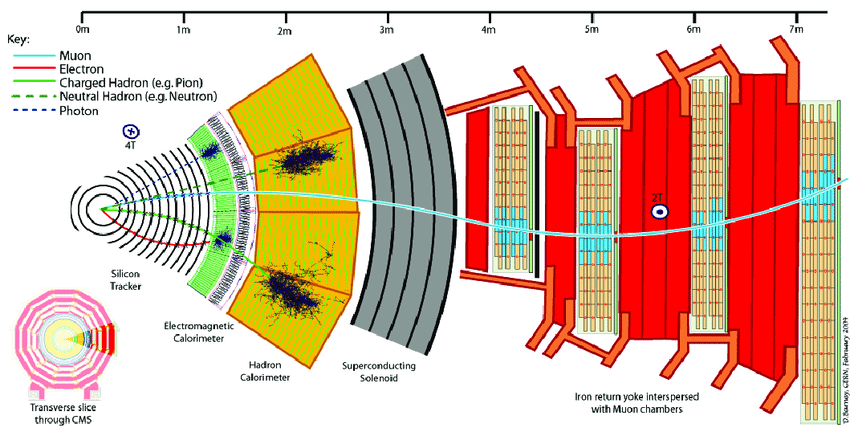
\includegraphics[width=0.9\textwidth]{figures/cms_slice}
\caption{A slice of CMS depicting the trajectory of a charged particle and its deposits in the subdetectors.}
\label{fig:cms_slice}
\end{figure}

\section{Reconstructing of Charged Particles}


Charged particles are detected in the first layer of CMS, the silicone tracker. The particle tracks are reconstructed using a combinatorial track finder, which uses a randomly generated track to find the hits compatible with the detected charged-particle trajectory. 


\section{Reconstructing Electrons}

Although electrons are generally stopped in the ECAL, the tracker is useful for detecting electrons because there are still inefficiencies that arise when determining which ECAL energy deposits correspond to electrons. Electrons leave a track in tracker, and they deposit some of their energy in the tracker through the mechanism of bremsstrahlung radiation. When the electron reaches the ECAL, it deposits its energy as well as the energy of the radiating bremsstrahlung photons, which results in a supercluster in the ECAL which must be detected as coming from one electron. However this is difficult to do in practice, as energy deposits from other particles in the ECAL often overlap with the electron’s supercluster.

\section{Reconstructing Muons}

The CMS detector is built to reconstruct muons as accurately as possible. The muon reconstruction is very efficient, with 99\% of muons accurately reconstructed. There can be false positives in the PF reconstruction of a muon, since some hadrons can punch through and be detected in the muon system. With multiple subdectors able to identify muons, there are three ways muons are detected that allows for PF reconstruction of the muon. Muons that are reconstructed in the tracker alone are called “tracker muson”. Musons that are reconstructed only in the muon detectors - teh drift tubes or the cathode strip chambers - are called “standalone muons”. Muons that are reconstructed using all subdetectors are “global muons''. Global muon reconstruction is the most efficient of the muon reconstructions when the muon $p_T$ is greater than 10 GeV.


\section{Jets}

Jets are reconstructed using a clustering algorithm. The jet clustering algorithm used in this analysis is the anti-kt algorithm. The jets clustered by the anti-kt algorithm and with a radius parameter of R=0.4 are called AK4 jets. 

[desribe anti-kt algorithm]

The AK4 jets can be reconstructed from only the ECAL and HCAL clusters. These jets are referred to as Calo Jets. The AK4 jets reconstructed with all of the particle flow information are called PF Jets. The jets reconstructed using all of the particles produced by an MC event generator are called Ref Jets. 


A diagram of these PF, Calo, and Ref jets is shown in Figure \ref{fig:pfjet}.

\begin{figure}[h]
\centering
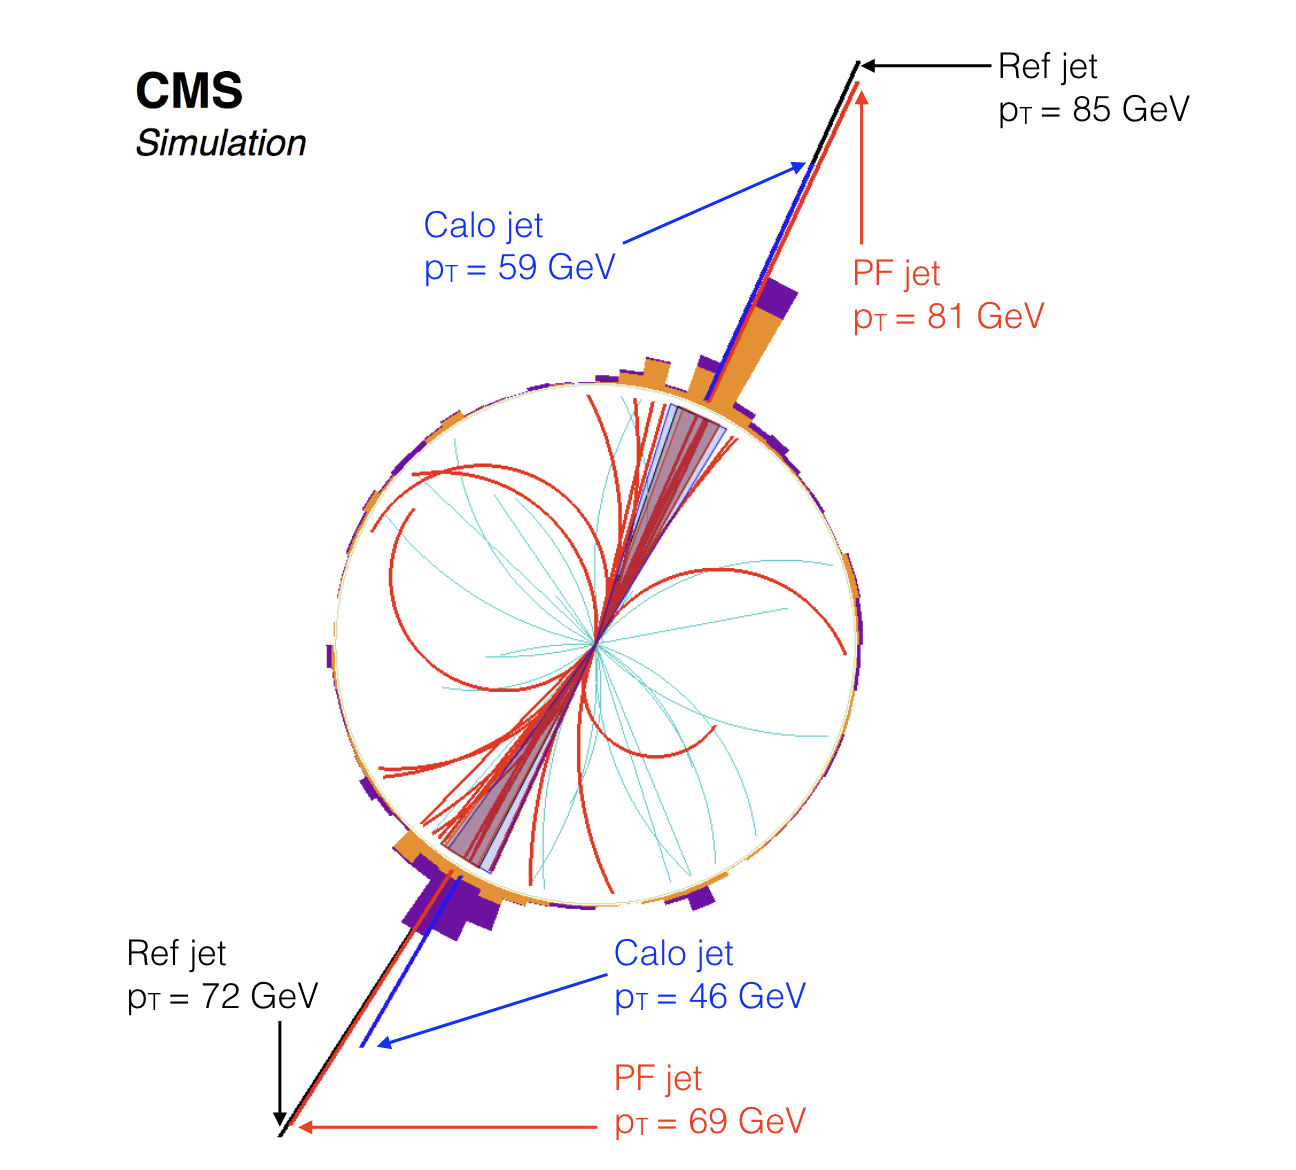
\includegraphics[width=0.9\textwidth]{figures/pf_jet_diagram}
\caption{A diagram of a dijet event and the reconstruction of the PF, Calo, and ref jets.}
}
\label{fig:pfjet}
\end{figure}

\section{Missing $E_T$}


\section{PF Validation}

